
%%******************************************************************************
%% SECTION - Materials 

%%******************************************************************************



\section{Bateria}
\label{bateria}


\begin{table}[ht!]

	\begin{tabular}{r l|l p{12cm} }
		
		\textcolor{gray}{Especificação} &&& 	{Bateria CSP Power CSP12 7 2 e
		Carregador Kita CM5A2}\\
		\textcolor{gray}{Data} &&& 				{28/05/2014}\\
        \textcolor{gray}{Beneficiado} &&&		{Ilha Baterias LTDA} \\
        \textcolor{gray}{CNPJ} &&& 				{42.453.779/0001-40} \\
        \textcolor{gray}{Número Nota} &&& 		{446} \\
		\textcolor{gray}{Quantidade} &&& 		{2 e 1} \\
		\textcolor{gray}{Valor} &&& 			{R\$270,00} \\
		\textcolor{gray}{Data Sheet} &&& 		{Anexo I - \ref{bateria}} \\

		\textcolor{gray}{Função no projeto} &&& {As baterias serão utilizadas dentro
		da eletrônica embarcada, como fonte de alimentação alternativa para os
		diversos dispositivos do projeto: sensores indutivos, sonares, sensores de
		inclinação e a eletrônica. O carregador é necessário caso a bateria
		descarregue durante os dias de teste.}
		\\
		\textcolor{gray}{Razão da Escolha} &&& {A bateria é de chumbo ácido, com
		pouco caráter explosivo e resistente a choque e curto circuito. O peso das
		baterias é maior, mas isso não é um fator limitante do projeto.}

	\end{tabular}
\end{table}

\newpage

\subsection{Foto do Material}
\begin{figure}[H]
 \centering
 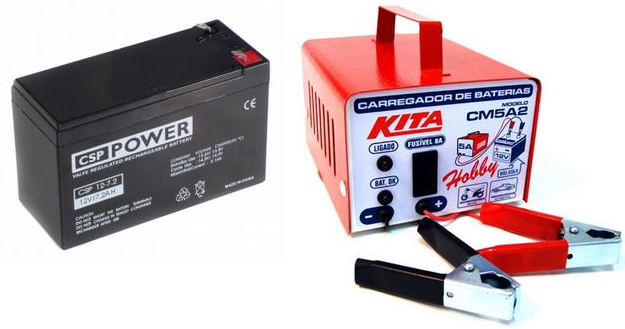
\includegraphics[width=1\columnwidth]{Bateria/foto.png}
 \caption{Bateria CSP Power e Carregador Kita}
\end{figure}

\subsection{Nota Fiscal}
\begin{figure}[H]
 \centering
 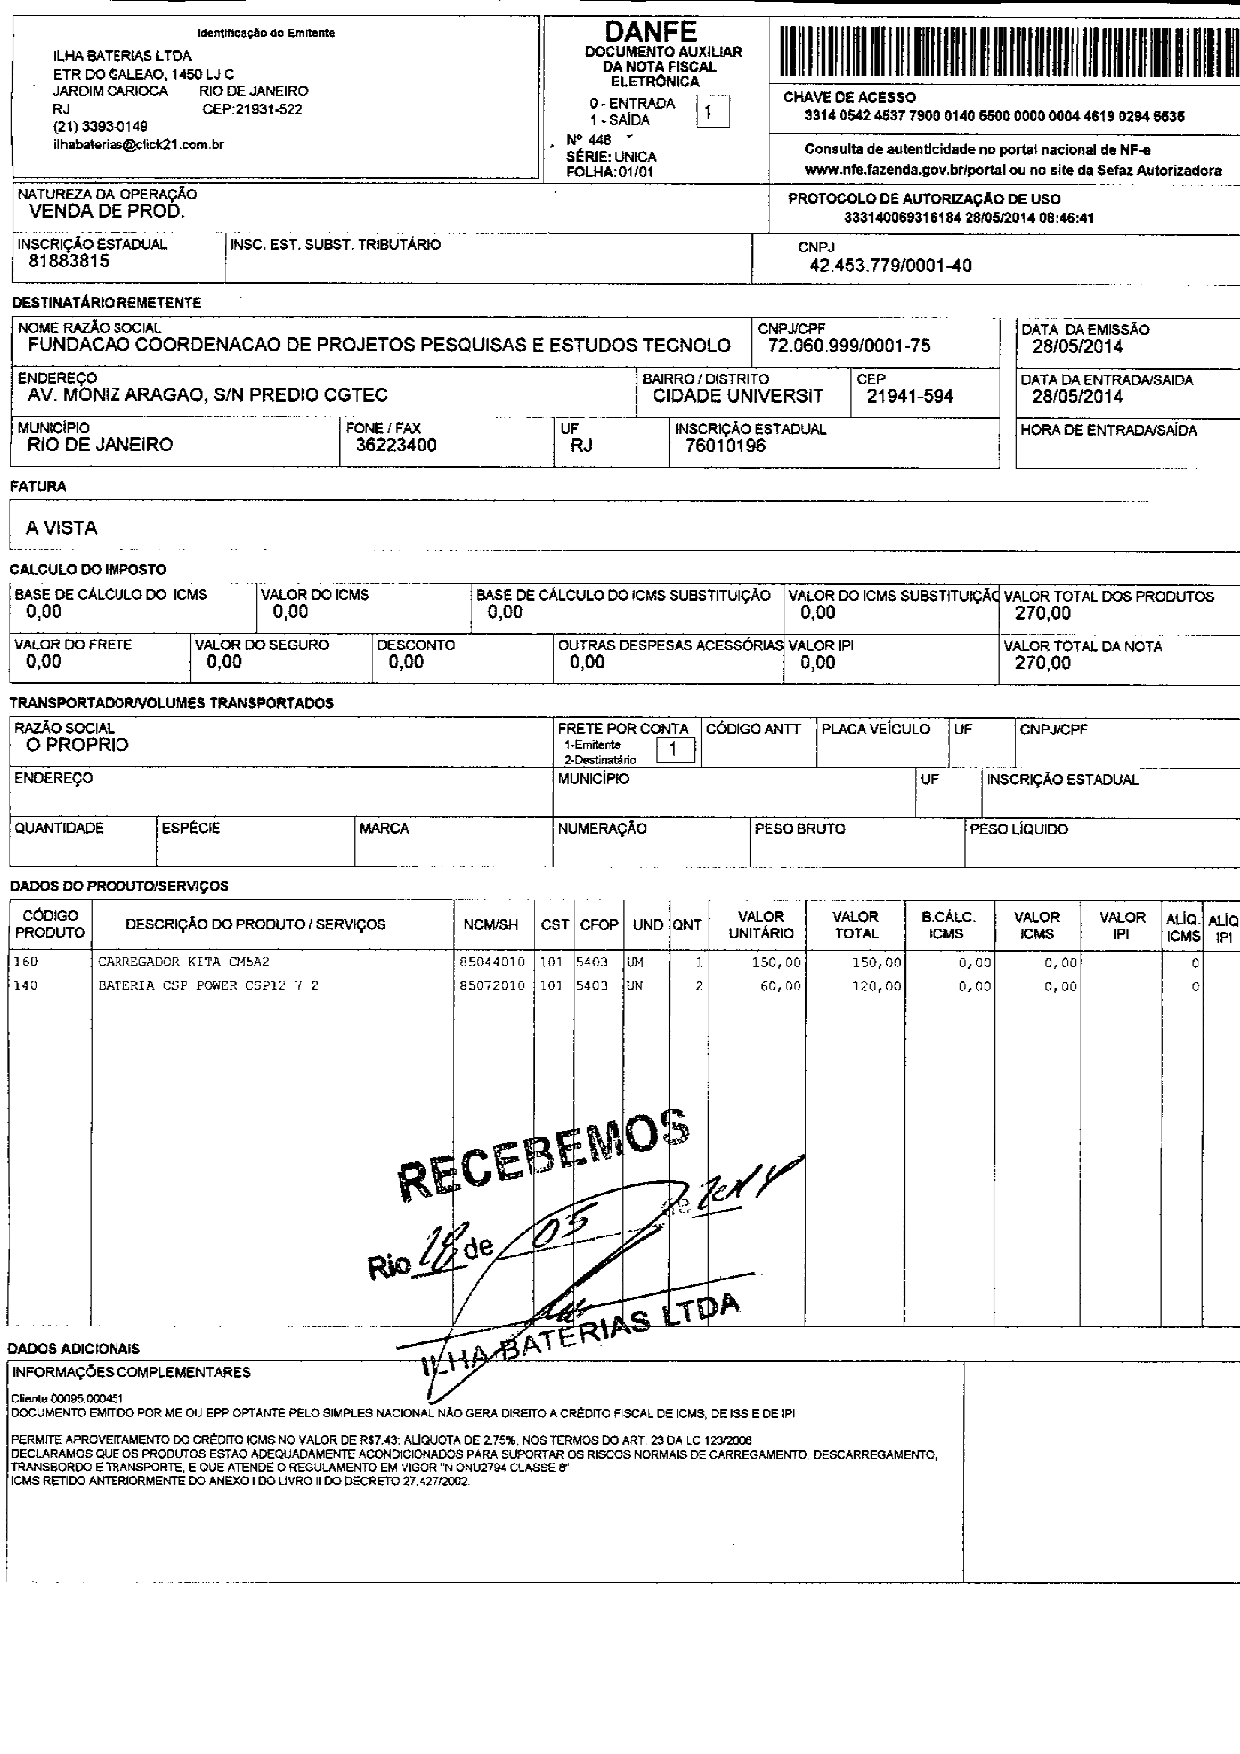
\includegraphics[width=0.9\columnwidth]{Bateria/nota_bateria.pdf}
 \caption{Bateria CSP Power CSP12 e Carregador Kita CM5A2 } 
 \end{figure}


